\documentclass[]{article}

\usepackage{
	amsmath, 
	amssymb,
	float,
	graphicx,
	bera,
	parskip
}

\graphicspath{ {Images/} }

\title{Assignment 4}
\author{
	Daniel Bok \\
	ESD \\
	1001049 \\
	daniel\_bok@mymail.sutd.edu.sg 
	\and
	Wong Yan Yee\\ 
	ISTD \\
	1001212 \\
	yanyee\_wong@mymail.sutd.edu.sg
	\and
	Clement Tan \\
	ESD \\
	1000948 \\
	clement\_tan@mymail.sutd.edu.sg
}
\date{\today}

\begin{document}
	
\maketitle

\newpage
\section*{Question 7.3}

\subsection*{A: Forming The Adjacency Matrix}

\begin{figure}[H]
	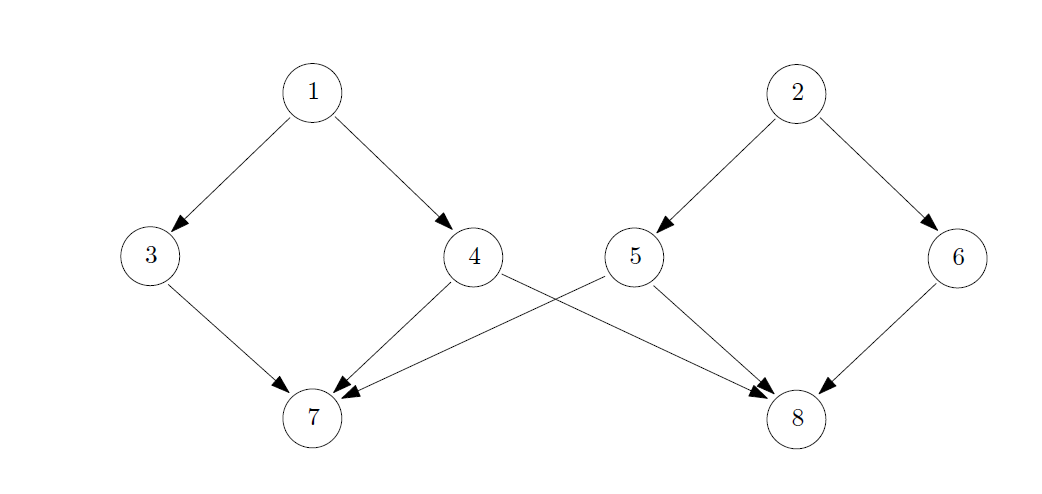
\includegraphics[width=\linewidth]{7-16.png}
	\caption{Network Graph} 
	\label{Q7.3 Network Graph 1}
\end{figure}

Given the network graph in Figure \ref{Q7.3 Network Graph 1}, the adjacency matrix $\mathbf{A}$ is given by
\begin{gather*}
	\mathbf{A} = \begin{bmatrix}
		0 & 0 & 1 & 1 & 0 & 0 & 0 & 0 \\
		0 & 0 & 0 & 0 & 1 & 1 & 0 & 0 \\
		0 & 0 & 0 & 0 & 0 & 0 & 1 & 0 \\
		0 & 0 & 0 & 0 & 0 & 0 & 1 & 1 \\
		0 & 0 & 0 & 0 & 0 & 0 & 1 & 1 \\
		0 & 0 & 0 & 0 & 0 & 0 & 0 & 1 \\
		0 & 0 & 0 & 0 & 0 & 0 & 0 & 0 \\
		0 & 0 & 0 & 0 & 0 & 0 & 0 & 0
	\end{bmatrix}
\end{gather*}

\subsection*{B: What is Matrix C?}

\begin{align*}
	\mathbf{C} &= \mathbf{A}^T\mathbf{A} \\
		&= \begin{bmatrix}
			0 & 0 & 0 & 0 & 0 & 0 & 0 & 0 \\
			0 & 0 & 0 & 0 & 0 & 0 & 0 & 0 \\
			0 & 0 & 1 & 1 & 0 & 0 & 0 & 0 \\
			0 & 0 & 1 & 1 & 0 & 0 & 0 & 0 \\
			0 & 0 & 0 & 0 & 1 & 1 & 0 & 0 \\
			0 & 0 & 0 & 0 & 1 & 1 & 0 & 0 \\
			0 & 0 & 0 & 0 & 0 & 0 & 3 & 2 \\
			0 & 0 & 0 & 0 & 0 & 0 & 2 & 3
		\end{bmatrix}
\end{align*}

The physical interpretation of $C_{ij}$ is the number of papers which cited paper $i$ and paper $j$ together. We notice that $C_{78} = C_{87} = 2$ because papers 4 and 5 cited both of them together. The same goes for $C_{56}$ and others.

We thus notice that $C_{78} > C_{75}$ because no papers which cited paper 5 cited paper 7 and vice versa. Thus $C_{75} = 0$.

\subsection*{C: Raising Matrix A}

\begin{align*}
	\mathbf{A}^2 &= \begin{bmatrix}
		0 & 0 & 0 & 0 & 0 & 0 & 2 & 1 \\
		0 & 0 & 0 & 0 & 0 & 0 & 1 & 2 \\
		0 & 0 & 0 & 0 & 0 & 0 & 0 & 0 \\
		0 & 0 & 0 & 0 & 0 & 0 & 0 & 0 \\
		0 & 0 & 0 & 0 & 0 & 0 & 0 & 0 \\
		0 & 0 & 0 & 0 & 0 & 0 & 0 & 0 \\
		0 & 0 & 0 & 0 & 0 & 0 & 0 & 0 \\
		0 & 0 & 0 & 0 & 0 & 0 & 0 & 0
	\end{bmatrix} \\
	\mathbf{A}^3 &= \begin{bmatrix}
		0 & 0 & 0 & 0 & 0 & 0 & 0 & 0 \\
		0 & 0 & 0 & 0 & 0 & 0 & 0 & 0 \\
		0 & 0 & 0 & 0 & 0 & 0 & 0 & 0 \\
		0 & 0 & 0 & 0 & 0 & 0 & 0 & 0 \\
		0 & 0 & 0 & 0 & 0 & 0 & 0 & 0 \\
		0 & 0 & 0 & 0 & 0 & 0 & 0 & 0 \\
		0 & 0 & 0 & 0 & 0 & 0 & 0 & 0 \\
		0 & 0 & 0 & 0 & 0 & 0 & 0 & 0
	\end{bmatrix}
\end{align*}

In general, the entries $a_ij$ in the matrix $\mathbf{A}^M$ refers to the number of ways to get from node $i$ to node $j$ in $M$ steps. $\mathbf{A}^3$ is a zero-matrix because there are no connections of length 3. 

\newpage

\end{document}
